% ------------------------------------------------------------------------ %
% !TEX encoding = UTF-8 Unicode
% !TEX TS-program = pdflatex
% !TEX root = ../Tesi.tex
% !TEX spellcheck = it-IT
% ------------------------------------------------------------------------ %
%
% ------------------------------------------------------------------------ %
% 	NOME APPENDICE 3
% ------------------------------------------------------------------------ %
%
\chapter{Conseus Process Flow}
%
\label{cap:conseus}
%
%
\begin{figure}[H]
	%
	\centering
	%
	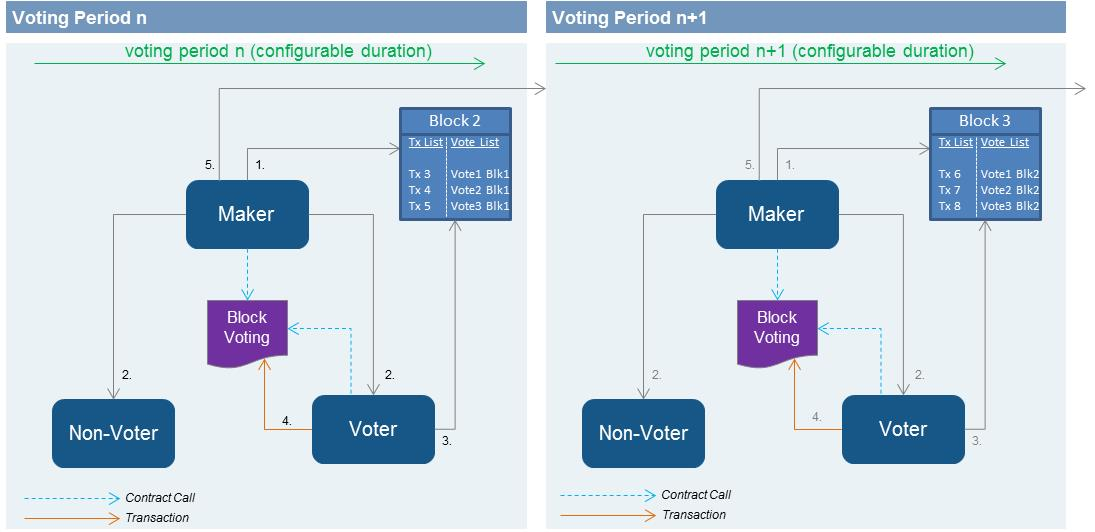
\includegraphics[width=.9\textwidth]{Quorum/conseus}
	%
	\caption{Flusso del consenso in Quorum}
	%
	\label{fig:flusso del consenso di quorum}
	%
\end{figure}
%
All'interno di un periodo:
\begin{enumerate}
	\item Il maker node che raggiunge il timeout per primo crea il blocco e lo firma. Il blocco include i voti per il blocco genitore che sono stati trasmessi nel precedente periodo.
	\item Il blocco viene pubblicato sulla rete utilzizando lo standard P2P Ethereum Protocol. Tutti i nodi ricevono il blocco, a prescindere dal loro ruolo.
	\item I Voters validano il blocco. Questo include:
	      \begin{enumerate}
	      	\item Chiamata al contratto BlockVoting per controllare se il maker può effettivamente creare il blocchi (i.e. ha il ruolo maker).
	      	\item Chiamata al contratto BlockVoting per controllare se il blocco genitore del blocco in valutazione ha ricevuto abbastanza voti.
	      	\item Vengono eseguite tutte le transazioni processabili nel blocco ovvero le transazioni pubbliche e quelle private del insieme di partecipanti di cui fa parte il nodo (questo dopo aver recuperato il payload transaciont dal Transaction Manager).
	      	\item Viene validato lo stato pubblico comparando il \emph{Public state root hash} con lo \emph{State root} all'interno del blocco.
	      	\item Viene effettuato l'hash di tutte le transazioni del blocco (sia pubbliche che private) e viene quindi confrontato con il \emph{transaction hash} del blocco. Questo viene realizzato per assicurarsi che tutti i Voters concordino sulla lista delle transazioni nel blocco.
	      \end{enumerate}
	\item Una volta validato con successo, i nodi Voters inviano il proprio voto al contratto BlockVoting usando una transazione Ethereum standard che viene distribuita su tutti i nodi. Dato che i voti per un dato blocco sono trasmessi tramite transazioni standard, possono essere processati solo quando il blocco successivo è stato creato.
	\item I maker node raggiungono il proprio timeout, determinano se il numero minimo di voti è stato raggiungo per il blocco precedente e poi la procedura di creazione del blocco$->$validazione$->$votazione viene ripetuta.
\end{enumerate}%
Mentre il consenso sullo stato privato è implicito e viene ottenuto attraverso una combinazione sincronizzata di input di contratti (\emph{Global Transaction Hash Validation Check}), un EVM deterministico (\emph{Public State Validation Check}), sincronizzazione della catena (nuovi blocchi aggiunti solo alla catena canonica) è possibile validare ulteriormente il consenso sullo stato privato tramite il comdanto Quorum \emph{eth\_StorageRoot}. Questo comando infatti restituisce il \emph{Private State Root Hash} di un account contratto ad un dato numero di blocco che può quindi essere validato rispetto al risultato dello storageRoot di una controparte fuori dalla catena o a livello di applicazione. Questa risulta un'ulteriore forma di sicurezza sulle transazioni private implementata dagli sviluppatori di Quorum. %
